\documentclass{article}

\usepackage{graphicx}
\usepackage{tikz}
\usepackage{tikzsymbols}
\usetikzlibrary{calc,patterns,shapes.geometric}
\pagestyle{empty}
\usepackage[margin=0pt]{geometry}
\geometry{papersize={14in,12in}}

\def\centerarc[#1](#2)(#3:#4:#5){\draw[#1] ($(#2)+({#5*cos(#3)},{#5*sin(#3)})$) arc (#3:#4:#5);}

\begin{document}
	\begin{figure}
		\centering
		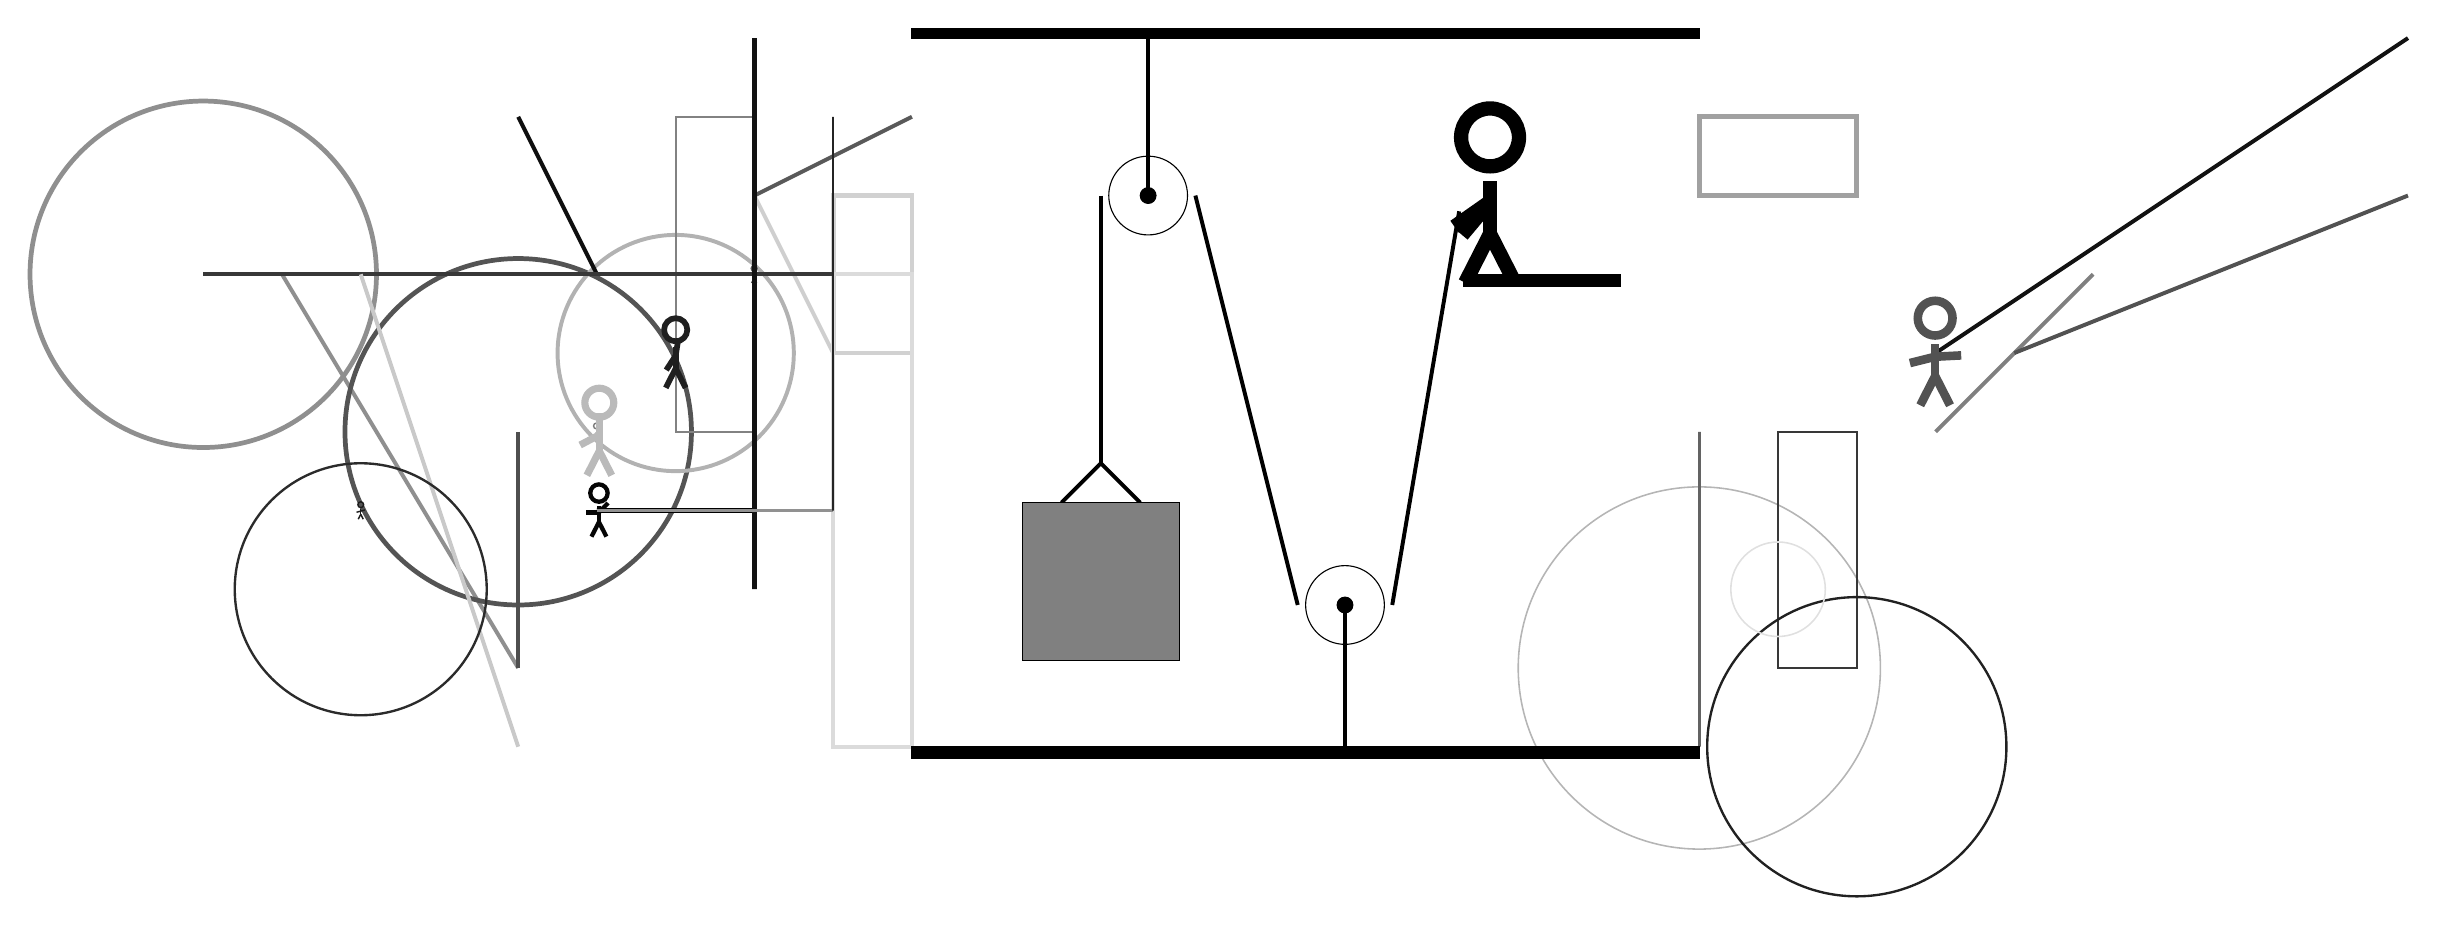
\begin{tikzpicture}
			%%%%% START %%%%%
			
			\draw[fill=black] (-2, 9) rectangle (8, 9.125);
			
			\draw (3.5, 1.8) circle (0.5);
			\draw[fill=black] (3.5, 1.8) circle (0.1);
			\draw[line width=0.5mm] (3.5, 1.8) -- (3.5, 0);
			
			\draw (1, 7) circle (0.5);
			\draw[fill=black] (1, 7) circle (0.1);
			\draw[line width=0.5mm] (1, 9) -- (1, 7);
			
			\draw[line width=0.5mm, color=black!44](-7, 1) -- (-10, 6);
			
			\draw[line width=0.5mm, color=black!19](-3, 5) -- (-4, 7);
			\draw [line width=0.6mm, color=black!67](-7, 4) circle (2.2);
			\draw[line width=0.6mm, color=black!37] (8, 7) rectangle (10, 8);
			\node[line width=0.3mm, color=black!51] at (-6, 4) {\Strichmaxerl[1][70][25]};
			\draw[line width=0.5mm, color=black!34](-7, 6) -- (-4, 6);
			
			\draw[line width=0.5mm, color=black!65](-2, 8) -- (-4, 7);
			\draw [line width=0.6mm, color=black!44](-11, 6) circle (2.2);
			\draw [line width=0.5mm, color=black!30](-5, 5) circle (1.5);
			
			\draw[line width=0.6mm, color=black!18] (-3, 5) rectangle (-2, 7);
			\draw [line width=0.2mm, color=black!29](8, 1) circle (2.3);
			\draw[line width=0.3mm, color=black!49] (-4, 8) rectangle (-5, 4);
			\draw[line width=0.3mm, color=black!78] (10, 1) rectangle (9, 4);
			\draw[line width=0.5mm, color=black!94](-7, 8) -- (-6, 6);
			\draw[line width=0.5mm, color=black!93](11, 5) -- (17, 9);
			\draw [line width=0.3mm, color=black!87](10, 0) circle (1.9);
			\draw[line width=0.3mm, color=black!61] (8, 0) rectangle (8, 4);
			\draw[line width=0.5mm, color=black!14] (-3, 0) rectangle (-2, 6);
			\node[line width=0.6mm, color=black!27] at (-6, 4) {\Strichmaxerl[5][28][90]};
			
			\draw[line width=0.7mm, color=black!100] (-4, 3) rectangle (-6, 3);
			\node[line width=0.7mm, color=black!67] at (-4, 6) {\Strichmaxerl[1][89][35]};
			
			\draw[line width=0.5mm, color=black!50](13, 6) -- (11, 4);
			\draw[line width=0.5mm, color=black!78](-3, 6) -- (-11, 6);
			\node[line width=0.7mm, color=black!98] at (-6, 3) {\Strichmaxerl[3][0][46]};
			\draw[line width=0.5mm, color=black!68](12, 5) -- (17, 7);
			\draw[line width=0.7mm, color=black!93] (-4, 2) rectangle (-4, 9);
			\draw[line width=0.5mm, color=black!69](-7, 4) -- (-7, 1);
			\node[line width=0.4mm, color=black!68] at (11, 5) {\Strichmaxerl[6][14][3]};
			
			\draw[line width=0.5mm, color=black!43](-3, 3) -- (-6, 3);
			\draw[line width=0.3mm, color=black!86] (-3, 8) rectangle (-3, 3);
			\node[line width=0.5mm, color=black!88] at (-5, 5) {\Strichmaxerl[4][57][81]};
			
			\draw[line width=0.5mm, color=black!21](-7, 0) -- (-9, 6);
			\node[line width=0.7mm, color=black!89] at (-9, 3) {\Strichmaxerl[1][15][16]};
			\draw [line width=0.2mm, color=black!12](9, 2) circle (0.6);
			\draw [line width=0.3mm, color=black!83](-9, 2) circle (1.6);
			
			\draw[line width=0.5mm](-0.1, 3.1) --  (0.4, 3.6) -- (0.9, 3.1);
			\draw[fill=black!50] (-0.6, 3.1) rectangle (1.4, 1.1);
			
			\draw[line width=0.5mm](0.4, 7) -- (0.4, 3.6);
			\centerarc[line width=0.5mm](1, 7)(180:0:0.6)
			\draw[line width=0.5mm](1.6, 7) -- (2.9, 1.8);
			\centerarc[line width=0.5mm](3.5, 1.8)(180:360:0.6)
			\draw[line width=0.5mm](4.1, 1.8) -- (4.95, 6.8);
			
			\node at (5.3, 7) {\Strichmaxerl[10][35][-130]};
			\draw[fill=black] (5, 6) rectangle (7, 5.85);
			
			\draw[fill=black] (-2, 0) rectangle (8, -0.15);
			
			%%%%% END %%%%%
		\end{tikzpicture}
	\end{figure}	
\end{document}